\documentclass{article}
\usepackage[portuges]{babel}
\usepackage[utf8]{inputenc}
\usepackage[T1]{fontenc}
\usepackage{graphicx}

\usepackage{float}
\usepackage{enumerate}
\usepackage{makeidx}
\usepackage{booktabs}
\usepackage{pdfpages}
\usepackage{a4wide}

\setlength\oddsidemargin{0.3in}
\setlength\evensidemargin{-0.3in}
\setlength\headsep{15pt}
\setlength\footskip{30pt}


% environment created for organization purposes, only.
\newenvironment{TODO}{%
  \color{blue} \itshape \begin{itemize}
}{%
  \end{itemize}
}

%---------------------------------------

% our addimage command
\newcommand{\addimg}[1]{%
  \begin{center}
    \includegraphics[width=0.75\textwidth]{#1}
  \end{center}
}

\newcommand{\RowStretch}[1]{\renewcommand{\arraystretch}{#1}}



%----------------------------------------------------------

\begin{document}

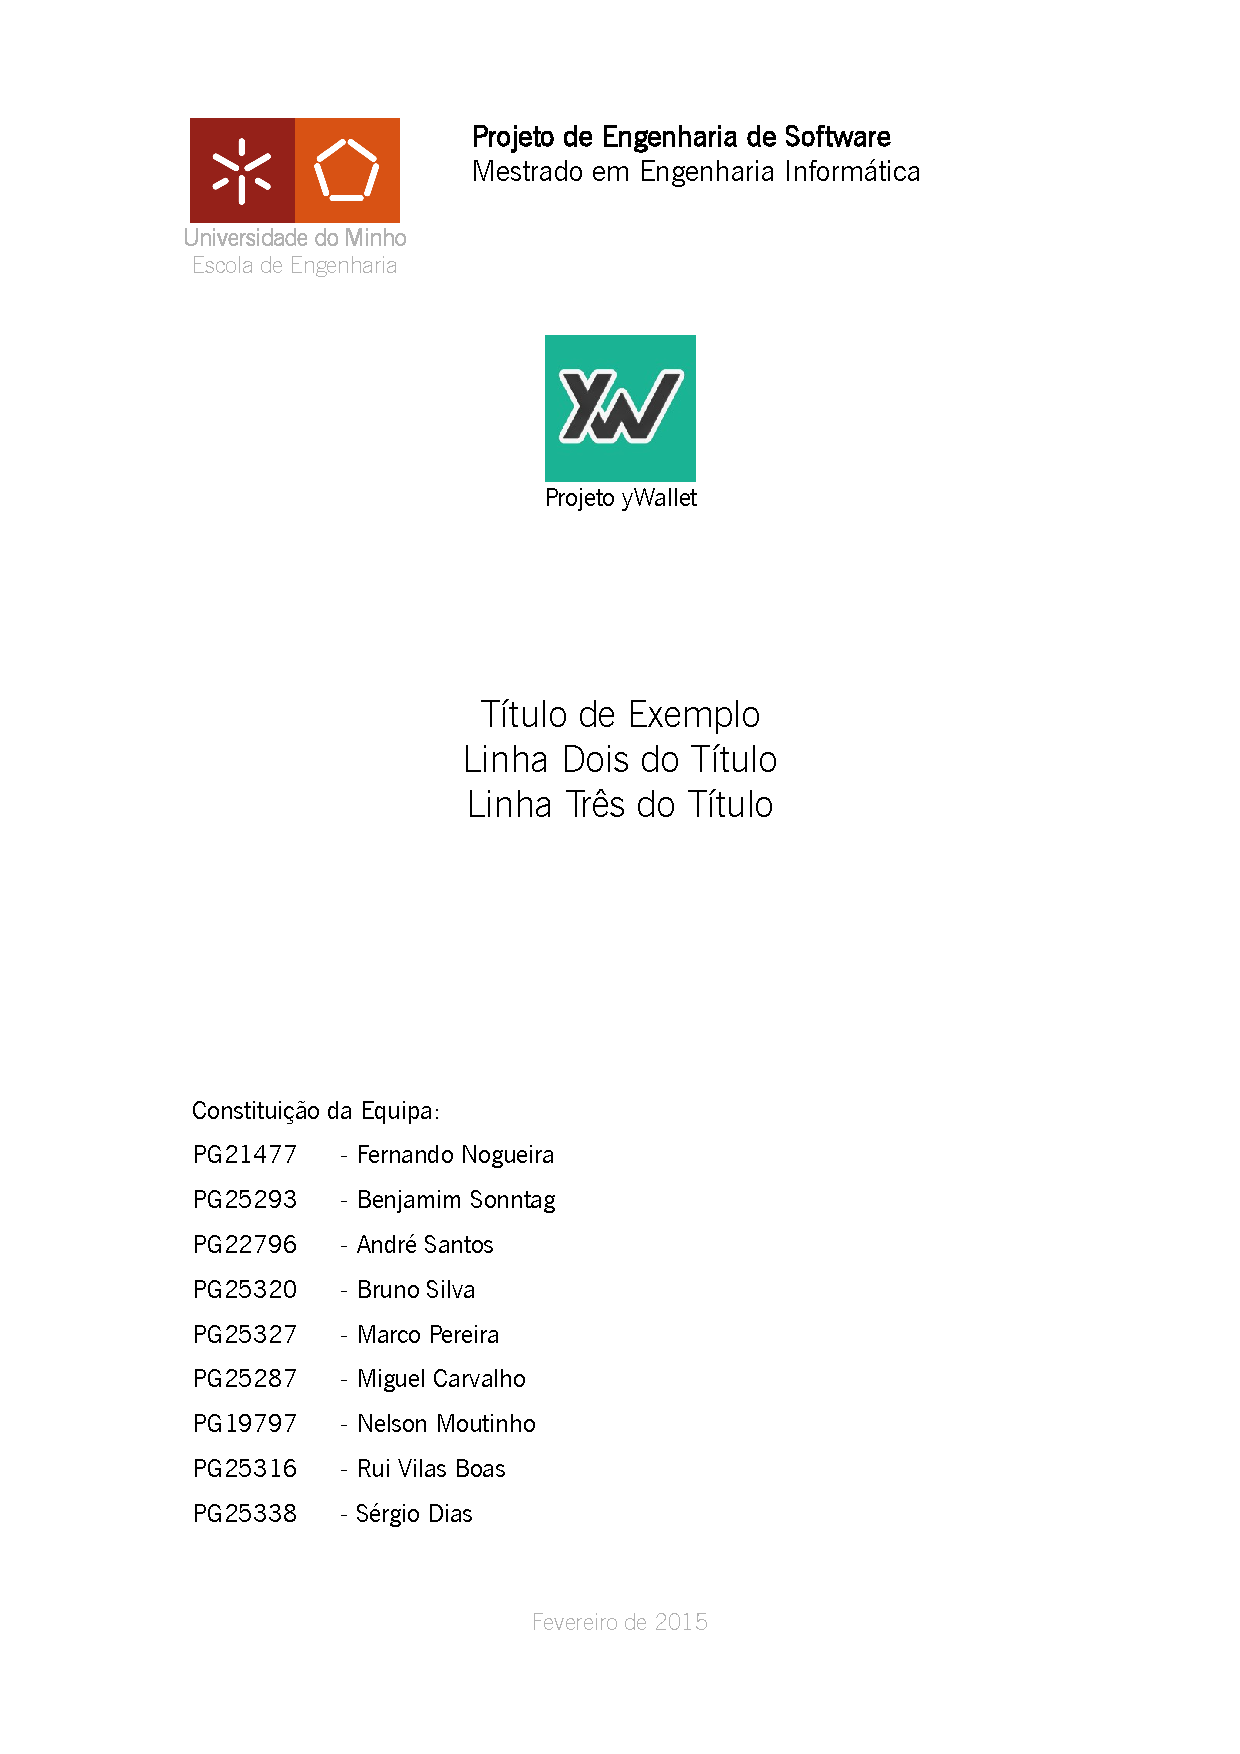
\includepdf[pages=-]{capa}

\tableofcontents

\section{Introduction}
\label{sec:introduction}
% \input{introduction}
Introdução do documento

\begin{table*}[ht]\centering
    \RowStretch{1.3}
    \begin{tabular}{@{}lccccccc@{}}\toprule
    Col1    & Col2  & Col3  & Col4  & Col5  & Col6 \\
    \midrule
    Val1    & Val2  & Val3  & Val4  & Val5  & Val6 \\
    \bottomrule
    \end{tabular}
    \caption{A sample table.}
    \label{tab:label}
\end{table*}

\end{document}
